\subsection{Transformación manual para vectorizar}


\subsubsection{\textbf{1ºBucle:}}
\par El primer bucle es \texttt{while(difference / (state.height * state.width) > tolerance)}. Se podría paralelizar creando una rama master y añadiendo un pragma de tipo
\texttt{task} que comparte la variable \texttt{iterations} antes del \texttt{if(verbose)} porque la ejecución de la siguiente iteración no depende de esto.
Además, dentro de esta \texttt{task} se necesita un pragma \texttt{atomic}, porque solo un hilo puede modificar a la vez esa variable global. Esta
implementación, mostrada en el código siguiente, no ayuda mucho en el rendimiento de la aplicación y la mejora es despreciable e incluso en 
algunos casos es peor como se indica en todas las tablas y gráficas.
%%% TABLA DE TIEMPOS E IMÁGENES %%%
\begin{figure}[H]
    \centering
    \begin{subfigure}{0.4\textwidth}
        \begin{adjustbox}{width=\textwidth} 
        \begin{tabular}{|c|c|c|c|c|}
            \hline
            \rowcolor{azul} \multicolumn{2}{|c|}{}&\multicolumn{3}{c|}{\textbf{Compiler}} \\ \hline
            \rowcolor{azul} \multicolumn{2}{|c|}{}&\texttt{clang}&\texttt{gcc}&\texttt{icc}\\ \hline
            \rowcolor{azul} \textbf{Testing size} & \textbf{Threads}&\multicolumn{3}{c|}{\textbf{Average time (s)}} \\ \hline
            \multirow{8}{1cm}{\textbf{01-small}} & 1 & \(1.58\pm{0.03}\) & \(0.32\pm{0.01}\) & \(1.00\pm{0.01}\) \\ \cline{2-5}
            & 2 & \(1.58\pm{0.03}\) & \(0.32\pm{0.01}\) & \(1.02\pm{0.01}\) \\ \cline{2-5}
            & 3 & \(1.60\pm{0.03}\) & \(0.33\pm{0.01}\) & \(1.02\pm{0.01}\) \\ \cline{2-5}
            & 4 & \(1.62\pm{0.01}\) & \(0.33\pm{0.01}\) & \(1.08\pm{0.04}\) \\ \cline{2-5}
            & 5 & \(1.62\pm{0.01}\) & \(0.33\pm{0.01}\) & \(1.05\pm{0.01}\) \\ \cline{2-5}
            & 6 & \(1.72\pm{0.01}\) & \(0.46\pm{0.01}\) & \(1.41\pm{0.35}\) \\ \cline{2-5}
            & 7 & \(1.99\pm{0.01}\) & \(0.47\pm{0.01}\) & \(1.44\pm{0.32}\) \\ \cline{2-5}
            & 8 & \(1.85\pm{0.01}\) & \(0.47\pm{0.02}\) & \(1.77\pm{0.02}\) \\ \hline
        \end{tabular}
        \end{adjustbox}
    \end{subfigure}
    \hfill
    \begin{subfigure}{0.5\textwidth}
        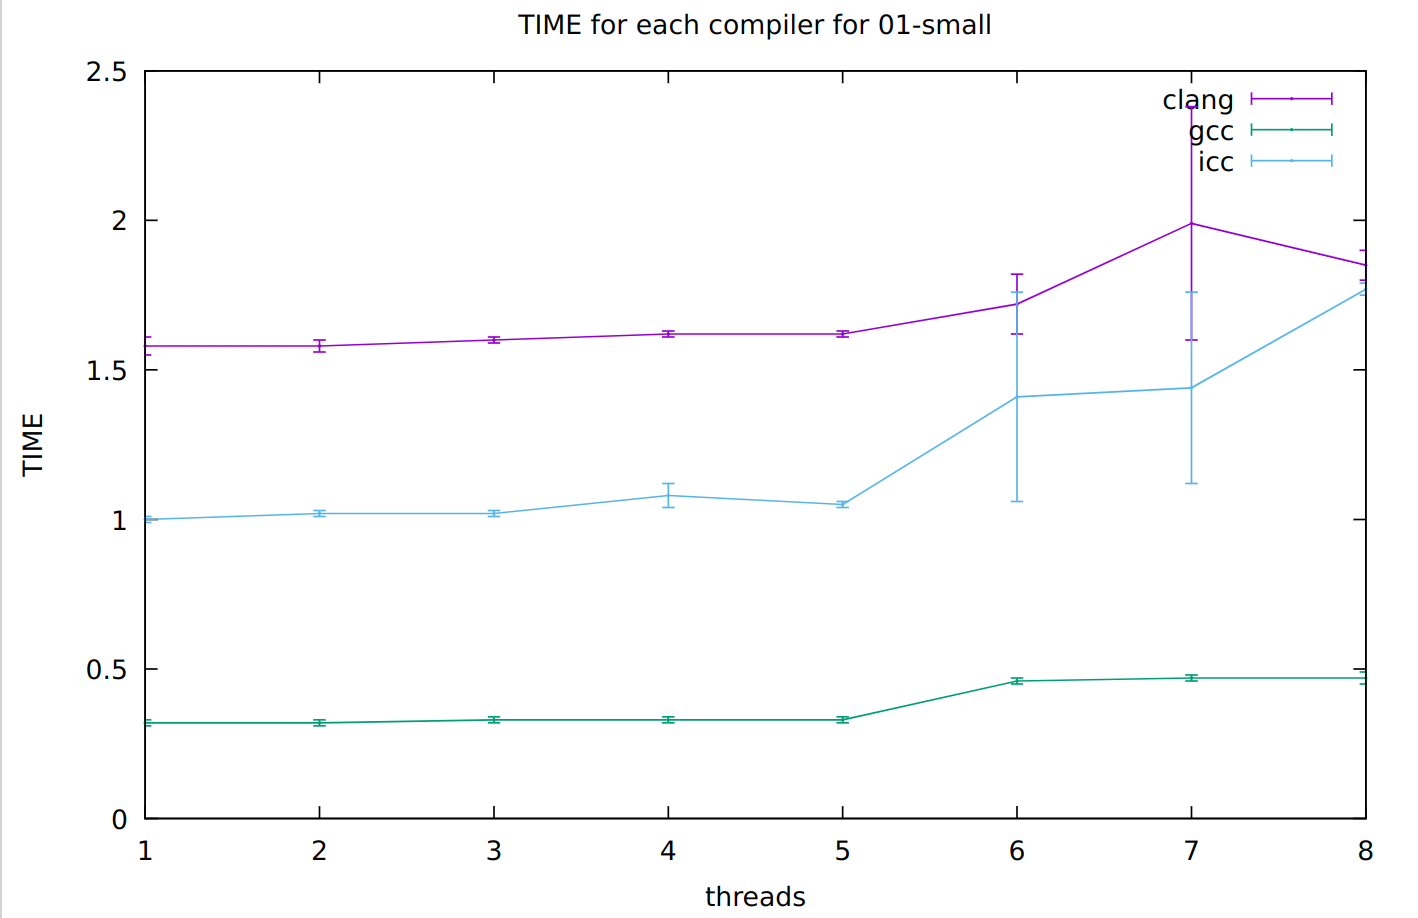
\includegraphics[width=\textwidth]{bucle1=01-small}
    \end{subfigure}
    \caption{\underline{1º Bucle, tamaño pequeño}: Tiempos de ejecución vs nº de hilos}
    \label{fig:bucle1=01-small}
\end{figure}
\newpage

\subsubsection{\textbf{heat.cpp}}
\begin{listing}[firstnumber=20]
    @@ -21,28 +21,36 @@
    void solve(Matrix<double>& state, double tolerance, int& iterations, double& last_difference) {
    Matrix<double> next_state = state;
    iterations = 0;
    double difference;
  + #pragma omp parallel
  + {
  + #pragma omp master
    do {
        difference = 0;
        for (size_t i = 1; i < state.height - 1; ++i) {
            for (size_t j = 1; j < state.width - 1; ++j) {
                next_state[i][j] = (state[i][j]
                                + state[i + 1][j]  
                                + state[i - 1][j]  
                                + state[i][j + 1]  
                                + state[i][j - 1]) / 5;
                difference = difference 
                             + abs(next_state[i][j]-state[i][j]);
            }
        }

        state.swap_data(next_state);

  + #pragma omp task shared(iterations)
  + {    
        if (verbose) {
            cout << "Iteration " << iterations << ":" << endl;
            printf_matrix("%7.3f", state);
            cout << "Difference: " << difference << endl;
        }
  + #pragma omp atomic
        ++iterations;
  + }
    } while (difference / (state.height * state.width) > tolerance);
    last_difference = difference / (state.height * state.width);
  + }
    }
\end{listing}


%%% TABLA DE TIEMPOS E IMÁGENES %%%
\begin{figure}[H]
    \centering
    \begin{subfigure}{0.4\textwidth}
        \begin{adjustbox}{width=\textwidth} 
        \begin{tabular}{|c|c|c|c|c|}
            \hline
            \rowcolor{azul} \multicolumn{2}{|c|}{}&\multicolumn{3}{c|}{\textbf{Compiler}} \\ \hline
            \rowcolor{azul} \multicolumn{2}{|c|}{}&\texttt{clang}&\texttt{gcc}&\texttt{icc}\\ \hline
            \rowcolor{azul} \textbf{Testing size} & \textbf{Threads}&\multicolumn{3}{c|}{\textbf{Average time (s)}} \\ \hline
            \multirow{8}{2.5cm}{\textbf{02-medium}} & 1 & \(4.83\pm{0.42}\) & \(0.89\pm{0.04}\) & \(2.88\pm{0.04}\) \\ \cline{2-5}
            & 2 & \(4.73\pm{0.24}\) & \(0.91\pm{0.04}\) & \(2.94\pm{0.04}\) \\ \cline{2-5}
            & 3 & \(4.57\pm{0.07}\) & \(0.90\pm{0.03}\) & \(3.22\pm{0.22}\) \\ \cline{2-5}
            & 4 & \(5.19\pm{0.57}\) & \(0.93\pm{0.04}\) & \(3.19\pm{0.21}\) \\ \cline{2-5}
            & 5 & \(4.63\pm{0.04}\) & \(1.28\pm{0.03}\) & \(3.16\pm{0.15}\) \\ \cline{2-5}
            & 6 & \(4.63\pm{0.03}\) & \(1.27\pm{0.03}\) & \(4.20\pm{0.86}\) \\ \cline{2-5}
            & 7 & \(4.64\pm{0.03}\) & \(1.27\pm{0.03}\) & \(4.83\pm{0.24}\) \\ \cline{2-5}
            & 8 & \(5.41\pm{0.08}\) & \(1.20\pm{0.04}\) & \(5.17\pm{0.10}\) \\ \hline
        \end{tabular}
        \end{adjustbox}
    \end{subfigure}
    \hfill
    \begin{subfigure}{0.5\textwidth}
        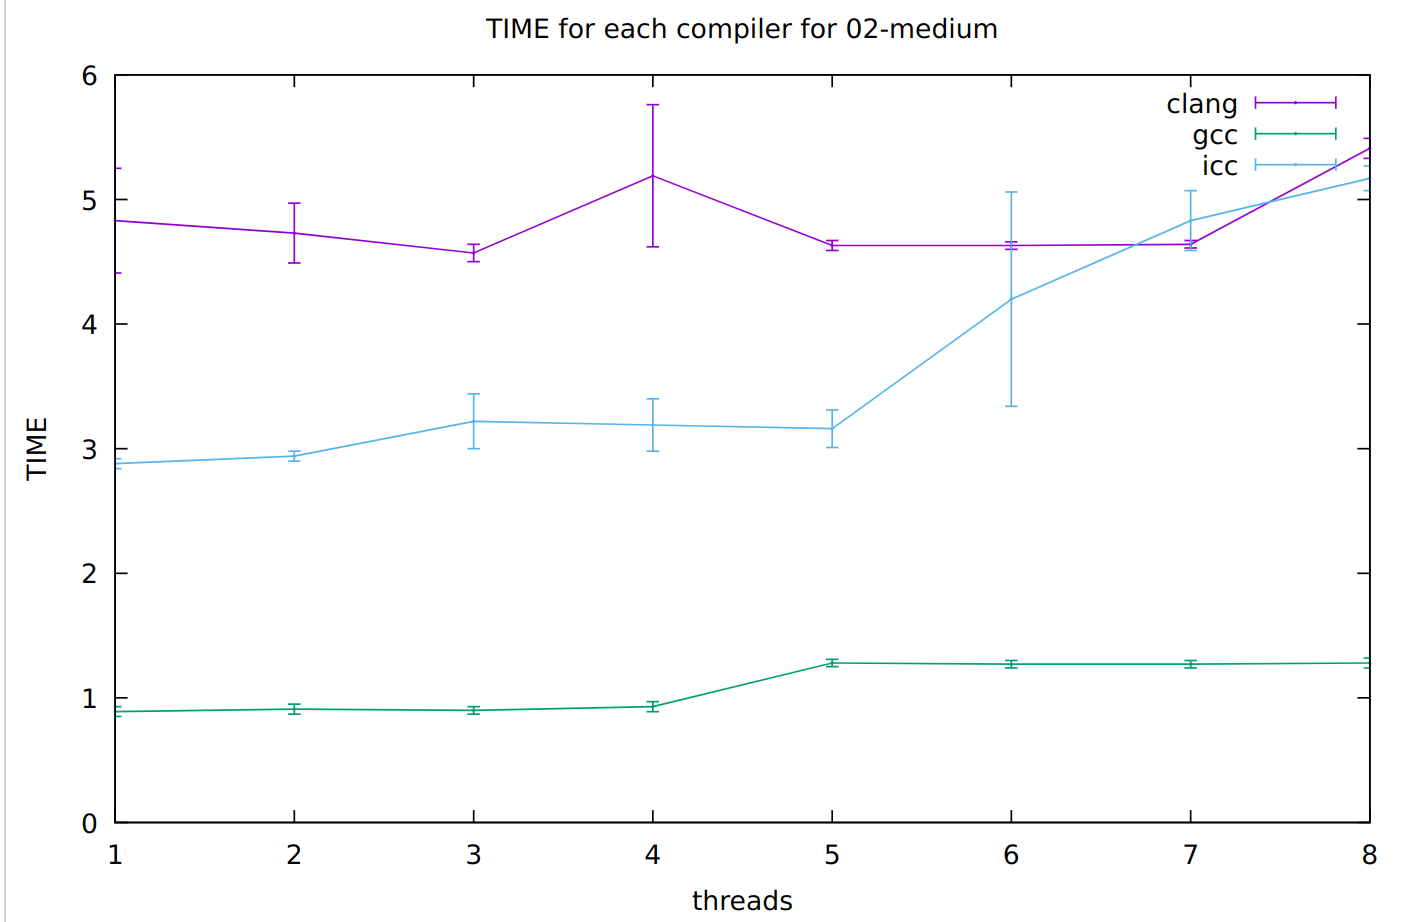
\includegraphics[width=\textwidth]{bucle1=02-medium}
    \end{subfigure}
    \caption{\underline{1º Bucle, tamaño mediano}: Tiempos de ejecución vs nº de hilos}
    \label{bucle1=02-medium}
\end{figure}

%%% TABLA DE TIEMPOS E IMÁGENES %%%
\begin{figure}[H]
    \centering
    \begin{subfigure}{0.4\textwidth}
        \begin{adjustbox}{width=\textwidth} 
        \begin{tabular}{|c|c|c|c|c|}
            \hline
            \rowcolor{azul} \multicolumn{2}{|c|}{}&\multicolumn{3}{c|}{\textbf{Compiler}} \\ \hline
            \rowcolor{azul} \multicolumn{2}{|c|}{}&\texttt{clang}&\texttt{gcc}&\texttt{icc}\\ \hline
            \rowcolor{azul} \textbf{Testing size} & \textbf{Threads}&\multicolumn{3}{c|}{\textbf{Average time (s)}} \\ \hline
            \multirow{8}{1cm}{\textbf{03-large}} & 1 & \(7.58\pm{0.01}\) & \(1.54\pm{0.11}\) & \(4.97\pm{0.13}\) \\ \cline{2-5}
            & 2 & \(7.69\pm{0.05}\) & \(1.55\pm{0.07}\) & \(5.11\pm{0.16}\) \\ \cline{2-5}
            & 3 & \(7.83\pm{0.01}\) & \(1.56\pm{0.08}\) & \(5.20\pm{0.21}\) \\ \cline{2-5}
            & 4 & \(7.87\pm{0.06}\) & \(1.61\pm{0.09}\) & \(5.23\pm{0.16}\) \\ \cline{2-5}
            & 5 & \(7.90\pm{0.03}\) & \(2.19\pm{0.05}\) & \(5.23\pm{0.18}\) \\ \cline{2-5}
            & 6 & \(7.87\pm{0.05}\) & \(2.17\pm{0.05}\) & \(5.20\pm{0.14}\) \\ \cline{2-5}
            & 7 & \(8.86\pm{0.01}\) & \(2.16\pm{0.06}\) & \(8.78\pm{0.18}\) \\ \cline{2-5}
            & 8 & \(8.85\pm{0.03}\) & \(2.15\pm{0.03}\) & \(8.76\pm{0.15}\) \\ \hline
        \end{tabular}
        \end{adjustbox}
    \end{subfigure}
    \hfill
    \begin{subfigure}{0.5\textwidth}
        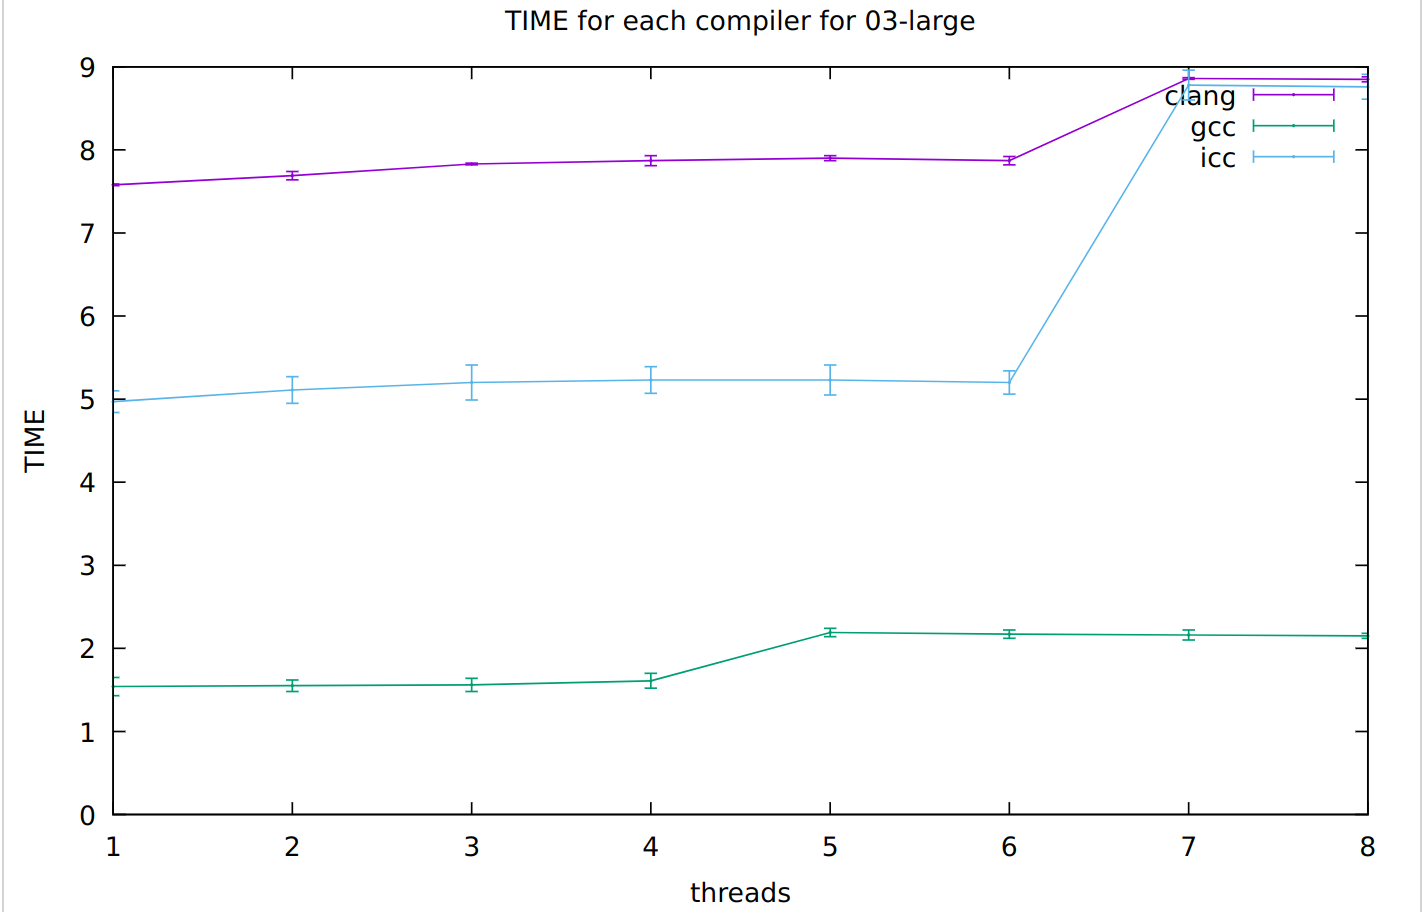
\includegraphics[width=\textwidth]{bucle1=03-large}
    \end{subfigure}
    \caption{\underline{1º Bucle, tamaño largo}: Tiempos de ejecución vs nº de hilos}
    \label{bucle1=03-large}
\end{figure}
\subsubsection{\textbf{3ºBucle:}}
\begin{listing}
    @@ -20,3 +20,4 @@
\end{listing}

\par El primer y tercer bucle no se pueden vectorizar de forma automática porque tiene dependencias. No son inmediatamente
vectorizables, tampoco se puede reorganizar el código para evitar las dependencias ni crear instrucciones parciales para mitigar la
dependencia. No he encontrado ninguna transformación manual para poder vectorizarlos. Separar cada bucle en dos sería
ineficiente y el compilador descarta la vectorización de la instrucción que ya no tendría dependencia por tanto este cambio no
sería una solución. A lo mejor se puede programar usando los instrinsics vectoriales, que son un conjunto de funciones
disponibles para lenguajes de alto nivel que corresponden directamente a instrucciones vectoriales o hay alguna librería
optimizada que ya esté vectorizada porque la idea de programar en lenguaje ensamblador hoy en día casi nunca se realiza.